\documentclass{article}
\usepackage{aaai}
\usepackage{fixbib}
\usepackage{amsmath}
\usepackage{graphicx}
\usepackage{times}
\usepackage{helvet}
\usepackage{courier}
\usepackage{graphicx}
\usepackage{verbatim}
\usepackage{url}
\graphicspath{ {images/} }
\frenchspacing
\setlength{\pdfpagewidth}{8.5in}
\setlength{\pdfpageheight}{11in}

\title{
	CS4246 Project 1\\ Depression Prediction
}
\author{
	{\bf Team 01} \\
	Antoine Charles Vincent Garcia - A0159072A\\
	Chan Jun Wei - A0112084\\
	Chen Tze Cheng - A0112092\\
	Eric Ewe Yow Choong - A0112204\\
	Han Liang Wee, Eric - A0065517\\
	Ho Wei Li - A0094679\\
}

\begin{document}
 	\maketitle

	\begin{abstract}
	\begin{quote}
	Depression is a worrying issue in modern times. If left unregulated, it can be dentrimental both health and life.
	
	In this report, we illustrate the use of Gaussian Processes (GP) to calculate and model stress levels in society and with the data obtained, is used to estimate depression severity. \\
	\end{quote}
	\end{abstract}
	
	\section{1. Introduction}
	For our experiment, we will use the GP model to measure and compute depression severity via audio recordings. We will also be discussing about the desirable properties of the GP model as well as the technical details such as the GP model requirements for the proposed application and modifications made to enhance performance. We will also include our experimental evaluations and procedure in this report.\\

	The rationale of depression prediction is enable authorities to take appropriate actions if an area or individual is depressed. For example, suicide and crime are often linked to high depression and stress levels. The data can help authorities to monitor and mitigate crime in areas with marked as 'depressed'. In addition, annual health checks may include psychiatrist recommendations which is given to individuals who falls into the depression category. If successful, these data can even be used to break down depression into 'levels' which are a better of measurement. \\

	\section{2. Gaussian Process Regression Model}
	As all individuals have varying inherent stress management, the use of the GP model for depression prediction makes use of all samples and feature information to perform the prediction including training data with different or uneven sampling rates. From the mean and variance obtained from previous data, we are able to predict if an individual is depressed. \\	

	\subsection{2.1 Qualitative Advantages}
	... \\

	\subsection{2.2 Important Requirements}
	 Our GP model requires multiple audio recordings of an individual's speech. \\

	\subsubsection{2.3 Energy}
	The Energy feature of a sound refers to the loudness of the sound at various timeframes, 
	hence it is obvious that energy of a sound is directly proportional to the amplitude of the soundwave. 
	This shows that the higher the energy, the louder the sound is going to be.	

	\subsubsection{2.4 Mel Frequency Cepstral Coefficients (MFCC)}: 
	Mel Frequency Cepstral (MFC) is a representation of short-term power spectrum of a sound, 
	based on a linear cosine transform of a log power spectrum on a nonlinear Mel scale of frequency. 
	MFCC are the coefficients that forms the MFC. The greatest benefit of using MFCC is that the scale approximates to the 
	human's auditory system response more closely, hence it allows for a better representation of sound. 
	In order to obtain MFCC, Fourier transformed is performed on the sound signals.	

	\subsubsection{2.5 Magnitude Spectrum}: 
	Magnitude spectrum can be produced by converting the input signal of an audio into frames. 
	Fast Fourier Transform (FFT) is performed on each frames and this will form the Magnitude Spectrum.
	
	\subsubsection{2.6 Zero-Crossing Rate}: 
	Zero crossing rate is the rate of sign-changes along a signal. This feature is extremely useful in speech recognition and music information retrieval.

	\subsection{2.7 Other Machine Learning Methods}
	Machine learning is about using model to learn from existing data for some improvement or prediction. 
	The following is some methods used in machine learning:

	\subsubsection{2.8 k-nearest neighbors algorithm}: 
	The k-Nearest Neighbors algorithm (or k-NN for short) is a non-parametric method used for classification and regression. 
	K is the user defined constant which classify the class of a vector data. The training examples are vectors in a multidimensional feature space, 
	each with a class label. The classification process of this algorithm can be visualize as the graph below.

	\subsubsection{2.9 Support Vector Machine (SVM)}: 
	Support Vector Machine (SVM), with the help of the libsvm, a developed library for SVM. 
	SVM is a type of linear classifiers that aims at finding a unique solution in the form of an optimal hyperplane. 
	This optimal hyperplane is defined as the one that maximizes the margins between the two classes. 
	It will be positioned at equal distance between the closest points of each class and will create the largest possible corridor with no points 
	from either classes inside. These closest points are on the border of the corridor and are called the support vectors.

	\subsubsection{2.10 Random Forest Regressor}: 
	Random Forest is an ensemble of decision trees, whereas a decision tree is trying to separate the data into different
	leaf nodes where the data points in each node have certain similarity. Each decision tree will predict a value and all of the values 
	will be averaged. The average value would be the prediction result.

	\subsubsection{2.11 AdaBoost}: 
	AdaBoost is the short form of Adaptive Boost. The output of the other learning algorithms ('weak learners') is combined 
	into a weighted sum that represents the final output of the boosted classifier. AdaBoost is adaptive in the sense that subsequent weak 
	learners are tweaked in favor of those instances misclassified by previous classifiers. AdaBoost first find out the classifier with the least errors, 
	then focus on those errors later by adding the weight to the outliers, then find out another classifier with least errors again. 
	The process is repeated till the end then all the classifier will be combined to form a final classifier which will indicate the class of data. 
	Therefore, AdaBoost is able to be sensitive to noisy data and outliers.

	\subsubsection{2.12 Naive Bayes}: 
	Naive Bayes is a prediction algorithm that uses Bayes rule in assumption of all naive Bayes classifiers assume that the value of a particular feature is 
	independent of the value of any other feature, given the class variable. Naive Bayes multiplies all the possibilities of a particular event occurs, then 
	give the prediction of possibility that event. All the data are extracted from the dataset to represent the possibilities which are the number of times 
	the particular event occurs in the dataset over the total number of events. Naive Bayes can produce great results if the features in the dataset is as 
	independent as possible. 

	\section{3. Technical Approach}
	\subsection{Application of Gaussian Process model}
	
	\textbf{Using Gaussian Process model as a machine learning model}: 
	When a person is depressed, no matter what time the person talks, we should also be able to determine the person is depressed according 
	to the speech signal. And we assume that the speech signals extracted from different depreessed people should be similar and thus is suitable 
	to use Gaussian Process Model.

	\subsection{Some Famous Mathematical Formula}
	\subsubsection{Euclidean Distance}
	Euclidean Distance is used to find the distance between two points in an Euclidean Space. Euclidean Distance is defined as:
	\begin{equation}\label{eq:eucdis}
		||x-x'|| = \sqrt{(x_{1} - {x_{1}}')^{2} + (x_{2} - {x_{2}}')^{2} + ... + (x_{n} - {x_{n}}')^{2}}  
	\end{equation}

	\subsubsection{Squared Euclidean Distance}
	It is just the squared of Euclidean Distance. Nothing special.
	\begin{equation}\label{eq:sq_eucdis}
		||x-x'||^{2} = (x_{1} - {x_{1}}')^{2} + (x_{2} - {x_{2}}')^{2} + ... + (x_{n} - {x_{n}}')^{2}  
	\end{equation}

	\subsection{Kernels}
	A general name for a function k of two arguments mapping a pair of inputs \( x \epsilon X, x' \epsilon X\) into R is a kernel.
	In other word, the similarity measure of all features is usually called kernel.\\
	This term arises in the theory of integral operators, where the operator \(T_{k}\) is defined as
	\begin{equation}\label{eq:Kernel_Tk}
		(T_{k}f)(x) = \int_{X} k(x,x') f(x') d\mu(x'),
	\end{equation}
	where \(\mu\) denotes a measure. A real kernel is said to be symmetric if k(x,x') = k(x',x); 
	clearly covariance functions must be symmetric from the definition.\\\\
	
	For a kernel to be used in Gaussian Process, one kernel must be  positive semidenite:\\
	A real n x n matrix K which satisfies 
	\begin{equation}\label{eq:psd_mat}
		\text{Q(v)} = v^{T}Kv \geq 0 \text{, } \forall v  \epsilon R^{n}
	\end{equation}
	is called positive semidefinite (PSD). 
	If Q(v) = 0 only when v = 0 the matrix is positive definite. Q(v) is called a quadratic form. 
	A symmetric matrix is PSD if and only if all of its eigenvalues are non negative. A Gram matrix corresponding to a covariance function is PSD.\\\\

	A kernel is said to be positive semidefinite if 
	\begin{equation}\label{eq:psd_kernel}
		\int_{}^{} \text{k(x,x')f(x)f(x')d}\mu\text{(x) d}\mu\text{(x')} \geq 0 \text{, } \forall f  \epsilon L_{2}\text{(X,}\mu\text{)}
	\end{equation}
	Equivalently a kernel function which gives rise to PSD Gram matrices for any choice of n  N and D is positive semidefinite.\\\\

	The kernels that would be chosen as our kernel is shown below 
	(The kernels are assumed to be defined on two samples \( x = ( x_{1} x_{2} x_{3} ... x_{n} ) \) and 
	\( x' = ( {x_{1}}' {x_{2}}' {x_{3}}' ... {x_{n}}')\) ,  
	represented as feature vectors in some input space):\\
	\begin{enumerate}
		\item \textbf{Radial Basis Function (RBF)}\\
		The RBF kernel is defined as 
		\begin{equation}\label{eq:kernel_rbf}
			K(x,x') = \exp^{-\frac{||x-x'||^{2}}{2\sigma^{2}}}
		\end{equation}
		\(||x-x'||^{2}\) represents Squared Euclidean Distance 
		And \( \sigma > 0 \) can either be a scalar (isotropic variant of the kernel) or a vector with the same number of dimensions 
		as the inputs X (anisotropic variant of the kernel). \\
		It is also known as the “squared exponential� kernel. This kernel is infinitely differentiable, 
		which implies that GPs with this kernel as covariance function have mean square derivatives of all orders, 
		and are thus very smooth.\\
		
		\item \textbf{Matern}\\
		The class of Matern kernels is a generalization of the RBF and the absolute exponential kernel parameterized 
		by an additional parameter nu. The smaller nu, the less smooth the approximated function is. For nu=\(\infty\), 
		the kernel becomes equivalent to the RBF kernel and for nu=0.5 to the absolute exponential kernel. 
		Important intermediate values are nu=1.5 (once differentiable functions) and nu=2.5 (twice differentiable functions).\\

		\item \textbf{Dot Product}\\
		The Dot Product kernel is non-stationary and can be obtained from linear regression by putting N(0, 1) priors on the coefficients 
		of \(x_{d}\) (d = 1, . . . , D) and a prior of N(0, \(\sigma_{0}^{2}\)) on the bias. 
		The Dot Product kernel is invariant to a rotation of the coordinates about the origin, but not translations. 
		It is parameterized by a parameter \(\sigma_{0}^{2}\). For \(\sigma_{0}^{2} = 0\), 
		the kernel is called the homogeneous linear kernel, otherwise it is inhomogeneous. The kernel is given by
		\begin{equation}\label{eq:kernel_dp}
			K(x,x') = \sigma_{0}^{2} + x \cdot x'  
		\end{equation}
		\\

		\item \textbf{Constant Kernel}\\
		The constant Kernel just set the similar measures to be a constant. The kernel is given by:
		\begin{equation}\label{eq:kernel_const}
			k(x,x') = C   
		\end{equation}
		where C is a constant, \(C \epsilon R and C \geq 0\)
		\\

		\item \textbf{Compound Kernel}\\
		Kernel which is composed of a set of other kernels.
		\\

		\item \textbf{Exp-Sine-Squared Kernel}\\
		The ExpSineSquared kernel allows modeling periodic functions. 
		Therefore, it is also called Periodic Kernel.  
		It is parameterized by a length-scale parameter, \(l > 0\) and a periodicity parameter \(p > 0\). 
		The kernel given by:
		\begin{equation}\label{eq:kernel_ess}
			k(x,x') = \exp^{(\frac{-2 sin( \frac{\pi ||x - x'||}{p})}{l})^{2}}   
		\end{equation}
		where \(||x - x'||\) represents Euclidean Distance. \\

		\item \textbf{Rational Quadratic Kernel}\\
		The RationalQuadratic kernel can be seen as a scale mixture (an infinite sum) of RBF kernels with different characteristic length-scales. 
		It is parameterized by a length-scale parameter \(l > 0\) and 
		a scale mixture parameter \( \alpha > 0 \). The kernel given by:
		\begin{equation}\label{eq:kernel_rq}
			k(x,x') = (\frac{1 + ||x - x'||^{2})}{2 \alpha l^{2}})^{-\alpha}
		\end{equation}
		where \(||x-x'||^{2}\) represents Squared Euclidean Distance \\

		\item \textbf{Linear Kernel}\\
		Linear Kernel is a simpler kernel which can run efficiently. However, its linearity assumption is its downside.
		The kernel is given by:
		\begin{equation}\label{eq:kernel_linear}
			k(x,x') = x^{T} x'
		\end{equation}
		\\

		\item \textbf{White Kernel}\\
		The kernel is used to estimate the noise-level(\(\delta\)) of the input. 
		The kernel is given by:
		\begin{equation}\label{eq:kernel_noise}
			if x == x', k(x,x') = \delta ; \text{else 0}
		\end{equation}
		\\

		\item \textbf{Ornstein–Uhlenbeck Kernel}\\
		The kernel is given by:
		\begin{equation}\label{eq:kernel_ou}
			k(x,x') = \exp^{(\frac{-||x - x'||}{l})}
		\end{equation}
		where \(||x - x'||\) represents Euclidean Distance. \\

		\item \textbf{Sum}\\
		Sum-kernel k1 + k2 of two kernels k1 and k2.\\
	\end{enumerate}

	\subsection{Novel Modifications}
	\textbf{Using Gaussian Process model to optimize the parameters of the ensemble of different maching learning model}: 
	The outcome of different machine learning model should be similar and thus is suitable to put inside Gaussian Process model.

	\section{4. Evaluation}
	In order to test our Gaussian Process model, we conducted tests on data obtained from Audio/Visual Emotion Challenge and Workshop(AVEC 2016). The goal of AEVC is to weigh-in on the various approaches(visual, audio) used to recognize emotions under unambiguous conditions. AVEC 2016 provided 2 pieces of data as input: visual and auditory data. However, we would be reducing the scope of the experiment, limiting the experiment to only the auditory data. Two Sub-Challenges are lised in AVEC 2016. We are only interested in the Depression Classification Sub-Challenge, which requires participants to classify inputs by the PHQ-8 score.

	\subsection{4.1 Data}
	The depression data used in AVEC 2016 was obtained from the benchmarking database, the Distress Analysis Interview Corpus - Wizard of Oz(DAIC-WOZ). Data collected from DAIC-WOZ include audio and video recordings and the corresponsing PHQ-8 score[CITE:27](0-24), which is a frequently used self-report scheme to access severity of depression[CITE]. Henceforth, we would need to pre-process the auditory data before we use it in our Gaussian Process Model. The data is pre-processed as described in the Section [REF]. The distribution of the depression severity scores in both training and development set is given in Figure \ref{histogram_phq8}. The data provided are split into 2 sets: training and development. A summary of the data is given in Table \ref{summary_table}.
	\begin{figure}
 	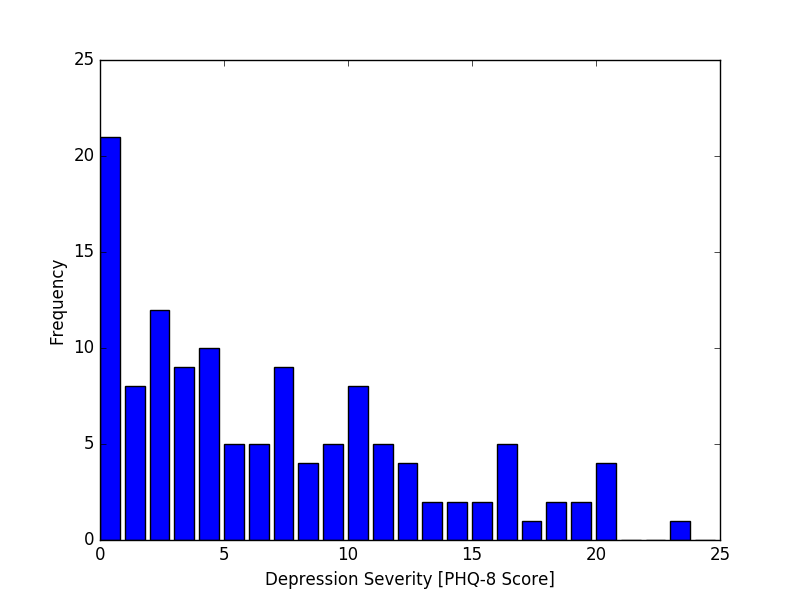
\includegraphics[width=0.45\textwidth]{histogram_phq8}
	\caption{PHQ-8 scores' histogram of both training and development set}
	\label{histogram_phq8}
	\end{figure}

 	\subsection{4.2	Measure of Accuracy}
	AVEC 2016 provided a baseline classifier that consistently predicts the PHQ-8 score with $\text{RMSE}=6.7418$[CITE]. In order to provide a meaningful and consistent comparison to the baseline provided, we would be only using Root Mean Square Deviation Error(RMSE) to measure the error rate on both Training and Development datasets. RMSE(Equation \ref{eq:rmse}) is a commonly used in machine learning communities to measure the differences between the values predicted by a model and the values actually observed. 

 	\begin{equation}\label{eq:rmse}
  	\text{RMSE} = \sqrt{\frac{\sum_{t=1}^n (\hat y_t - y_t)^2}{n}}
 	\end{equation}
 	\begin{table}
 		\begin{center}
  			\begin{tabular}{ | r | c | c || c | }
    			\hline
			 & Training & Development & All \\ \hline
			 n               & 95 & 31 & 126 \\ \hline
			 $\mu$           & 6.326 & 7.548 & 6.626 \\ \hline
			 $\sigma$        & 5.597 & 6.690 & 5.909 \\ \hline
			 \end{tabular}
		\end{center}
 	\caption{Summary of Datasets provided}
 	\label{summary_table}
 	\end{table}
 	[CITEDBLP:journals/corr/ValstarGSRLTSSC16]
 
	\subsection{4.3	Experimental Setup}
	We compared our Gaussian Model against commonly used machine learning algorithms. The list of algorithms and their hyperparameters are given in Table \ref{list_mls}. The hyper-parameters are either determined by the defaults used in the popular machine learning library, Scikit Learn[CITE] or some reasonable values were used. Each machine learning algorithm is trained against the training set and thereafter tested against the development set using RMSE as the error metric. The process used is shown in Figure \ref{process}.
	\begin{figure}
 		\begin{center}
		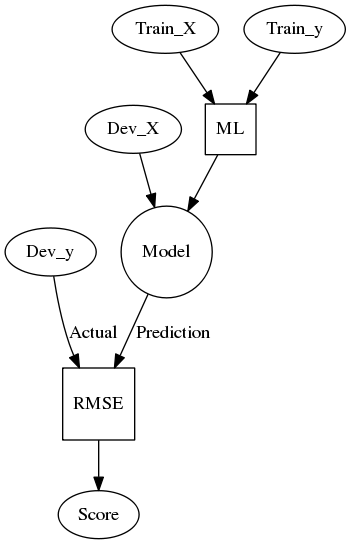
\includegraphics[width=0.25\textwidth]{process}
  		\end{center}
  		\caption{Experimental process}
  		\label{process}
 	\end{figure}
 	\begin{comment}
 	DO NOT REMOVE
	@startuml
 	digraph g {
	 	ML,RMSE[shape=square];
		Model[shape=circle];
		Train_X -> ML;
		Train_y -> ML;
		ML -> Model
		Dev_X -> Model
		Model -> RMSE[label=Prediction]
		Dev_y -> RMSE[label=Actual]
		RMSE -> Score
	}
 	@enduml
 	\end{comment}

 	\begin{table}
  		\begin{center}
   			\begin{tabular}{ | r | c |}
	    		\hline
			Algorithm & Hyper-parameters \\ \hline\hline
			K-Nearest Neighbors        & x \\ \hline
			Linear SVM                 & x \\ \hline
			RBF SVM                    & x \\ \hline
			Decision Tree              & x \\ \hline
			Random Forest              & x \\ \hline
			AdaBoost                   & x \\ \hline
			Naive Bayes                & x \\ \hline
			Decision Tree              & x \\ \hline
			\end{tabular}
		\end{center}
		\caption{List of Machine Learning Algorithms with their corresponding hyper-parameters}
		\label{list_mls}
	\end{table}
	
	\subsection{4.4	Results}
	The results of the experiment is shown in t
 
	\begin{table}
		\begin{center}
			\begin{tabular}{ | r | c | c |}
			\hline
			& \multicolumn{2}{c|}{RMSE} \\ \hline
			Algorithm & Training & Development \\ \hline\hline
			K-Nearest Neighbors        & x & x \\ \hline
			Linear SVM                 & x & x \\ \hline
			RBF SVM                    & x & x \\ \hline
			Decision Tree              & x & x \\ \hline
			Random Forest              & x & x \\ \hline
			AdaBoost                   & x & x \\ \hline
			Naive Bayes                & x & x \\ \hline
			Decision Tree              & x & x \\ \hline
			Gaussian Process           & x & x \\ \hline
			\end{tabular}
		\end{center}
		\caption{RMSE results of the different machine learning algorithms}
		\label{rmse_results}
	\end{table}
 
 	\begin{figure*}
	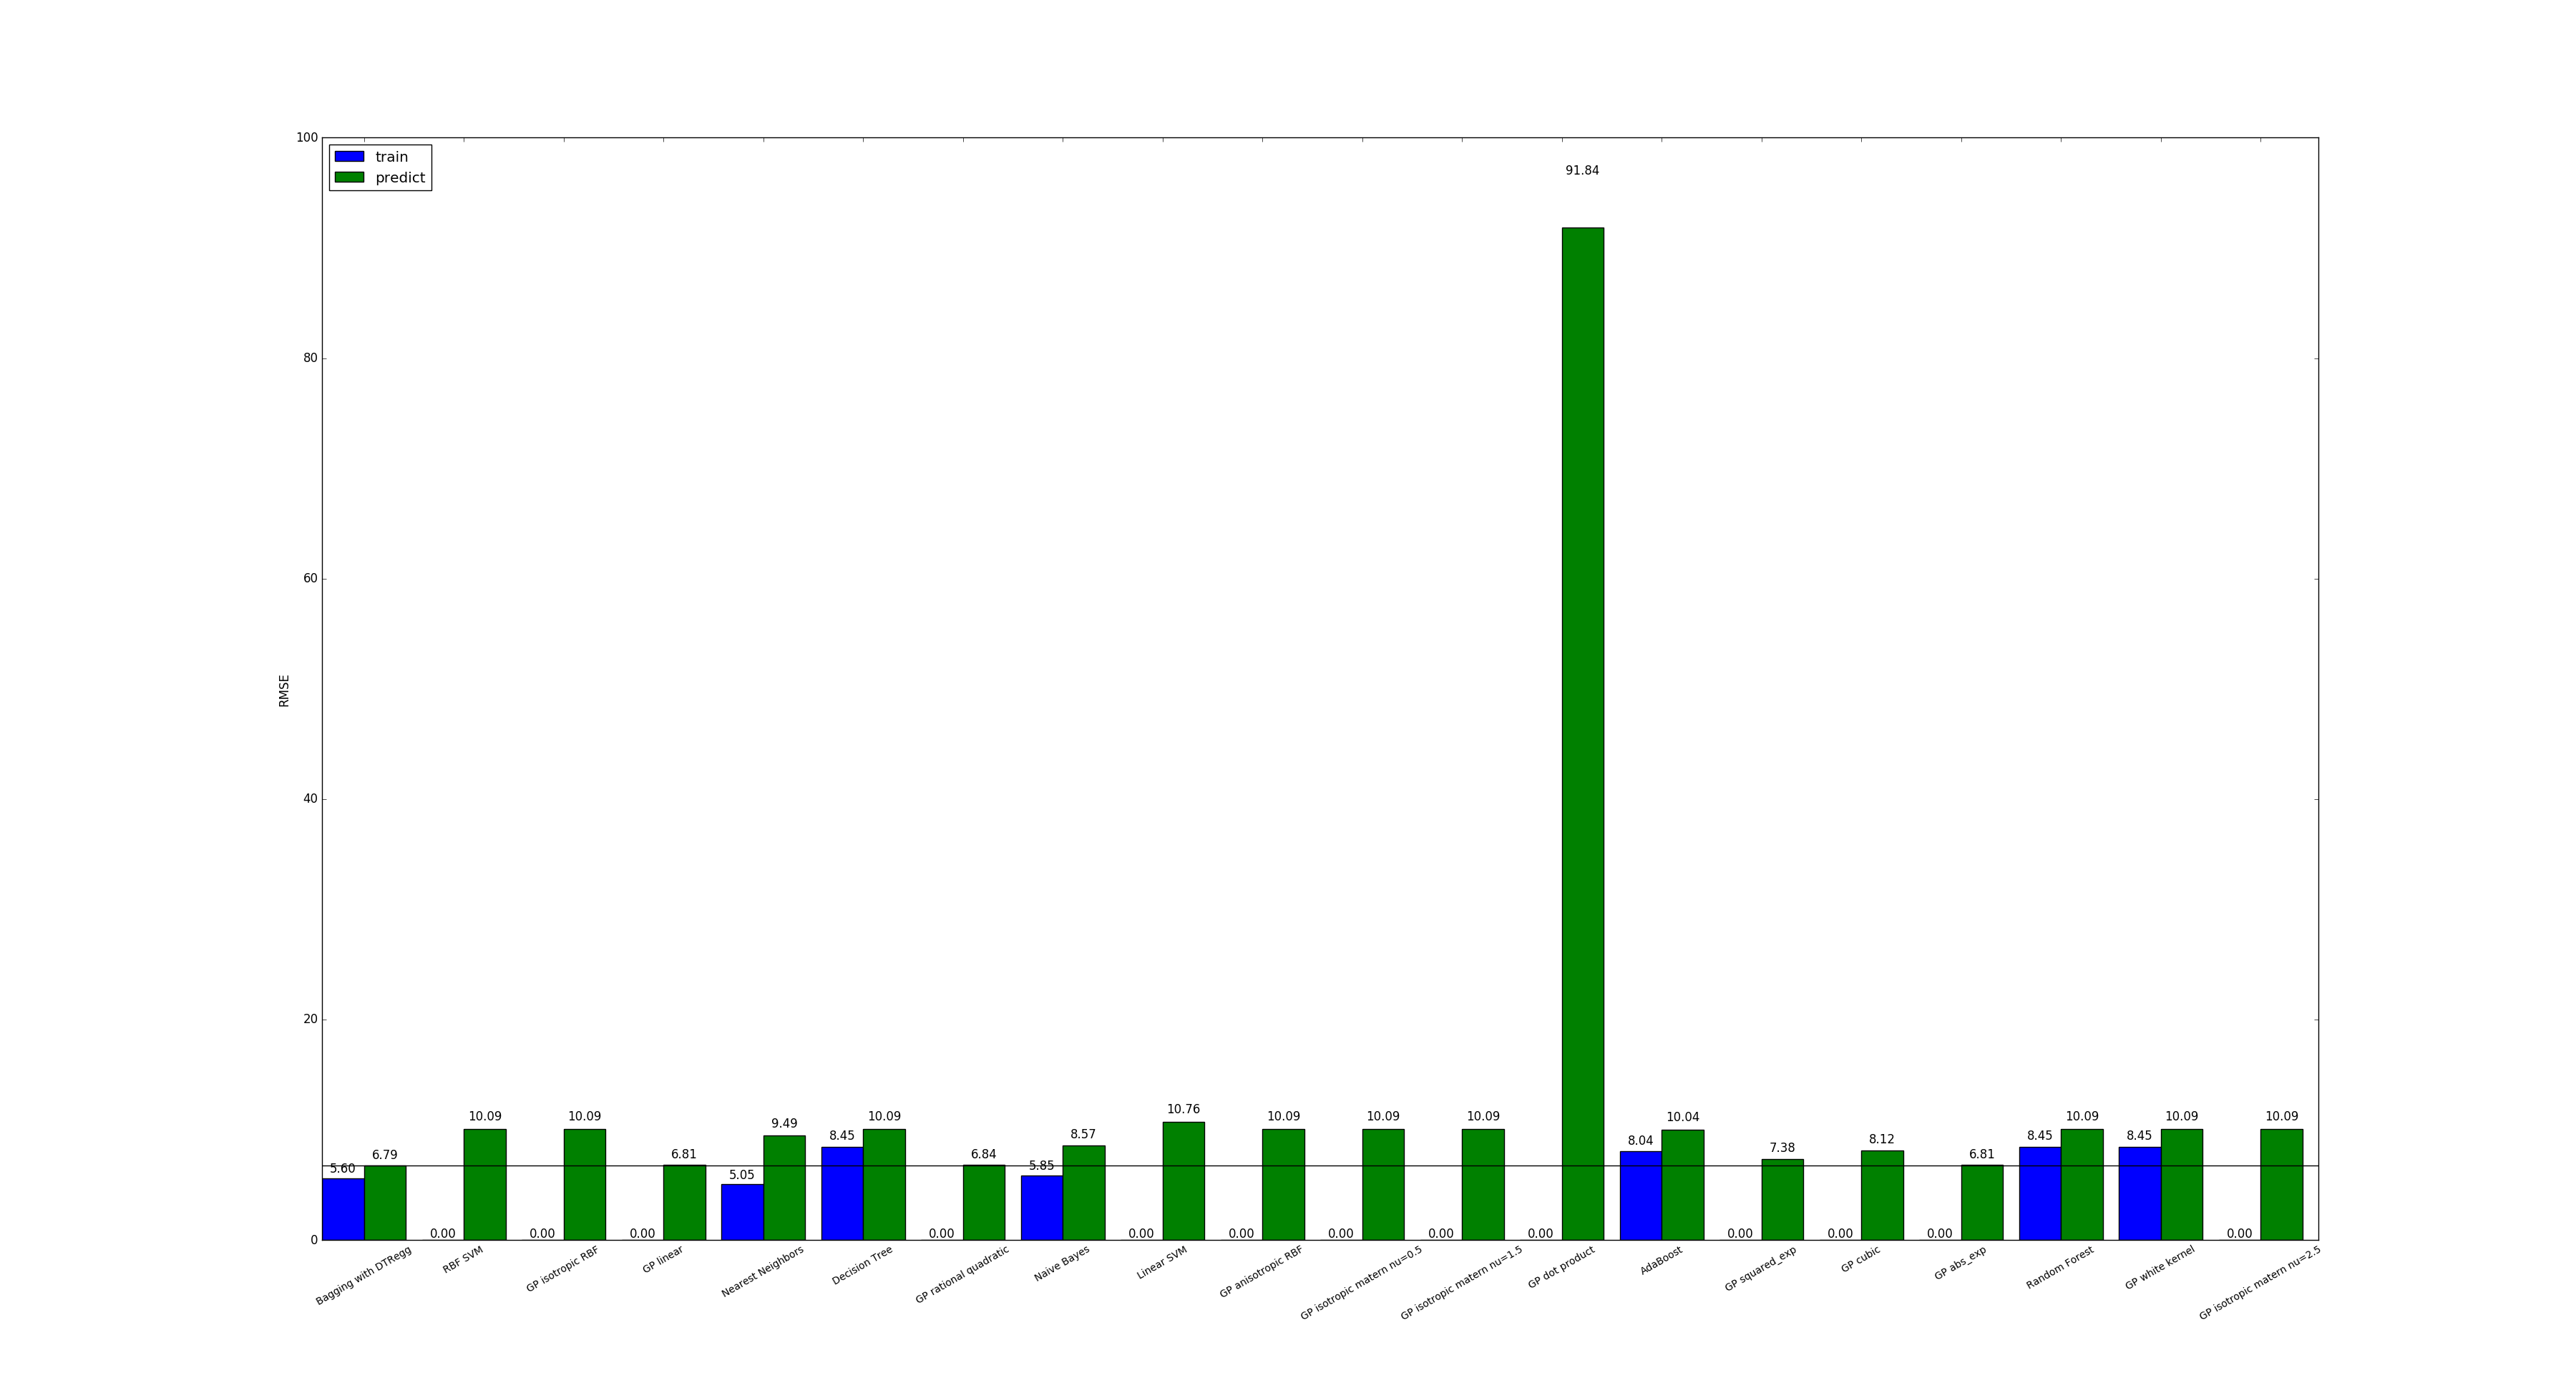
\includegraphics[width=\textwidth]{results}
	\caption{Chart showing RMSE(Training and Development) for the different classifiers}
	\label{rmse_results_chart}
	\end{figure*}

	\section{5. Conclusion}	
	... \\

	\section{6. Main Roles of Each Member}
	\begin{itemize}
		\item \textbf{Antoine Charles Vincent Garcia}: 
		Scripting the program, setting up machine learning libraries and running tests.
		\item \textbf{Chan Jun Wei}: 
		Project technicalities such as problem formulation and modelling, mathematics and experiment planning.
		\item \textbf{Chen Tze Cheng}: 
		Project technicalities such as problem formulation and modelling, mathematics and experiment planning.
		\item \textbf{Eric Ewe Yow Choong}: 
		Documentation especially writing of the motivation, recording research findings and keeping track of requirements.
		\item \textbf{Han Liang Wee, Eric}: 
		Scripting the program, setting up machine learning libraries and running tests.
		\item \textbf{Ho Wei Li}: 
		Documentation especially writing up the motivation, recording research findings and keeping track of requirements.
	\end{itemize}
	
	\bibliographystyle{aaai}
	\bibliography{references}

\end{document}